\chapter{Le problème} \label{chapPb}
	\section{Les tests} \label{pbTests}
	Comme expliqué dans la section \ref{besoinTests}, le calculateur moteur est un système critique, il est donc indispensable de tester correctement celui-ci.

	\subsection{Le plugin}
	Dans le cadre de projets pour Ford, Continental ne développe pas l'intégralité du calculateur, en effet une partie est fournie par le client sous forme de << plugin >>. Le plugin est supposé correct, et ce n'est pas du ressort de continental de le tester. Cependant, celui-ci va être interfacé avec les logiciels Continental : il est indispensable de vérifier que les deux parties fonctionnent ensemble lors de l'intégration.

	Pour cela, le client fournis un fichier appelé \textit{Walkthrough}\footnote{Ce fichier est expliqué plus en détail section \ref{wt}} contenant la liste des variables du plugin avec toutes leur spécifications, ce fichier est au format Excel : environ 900 variables différentes. Il est impensable de tester le fonctionnement d'autant de paramètres << à la main >>, ainsi l'équipe en charge de tester cette intégration effectue des tests de différence d'une version à l'autre : seul les variables ayant pu être impacté par une \textit{release} seront testés, il est supposé que les autres resteront inchangées.

	Trois problèmes se posent à cette méthode : 
	\begin{description}
		\item[La fiabilité des tests] Rien ne nous garantie qu'une variable ne va pas être impacté par une modification, un problème peut donc passer à côtés du test.
		\item[Le temps de tests] Même en ne testant qu'une partie des variables, cela prend un temps considérable, il faut compter environ une semaine pour tester ce qu'il faut, sans compter le fait qu'une tâche répétitive peut entrainer des erreurs d'inattention.
		\item[La disponibilité des bancs de tests]	Les tests s'effectuent sur des bancs de tests\footnote{Une photo d'un banc est disponible figure \ref{fig:photoHil}}, ces équipements permettent de simuler un environnement voiture autour du contrôleur moteur\footnote{tel que l'utilisation de la clé de démarrage, la tension de la batterie, la vitesse de rotation du moteur, ...} Or ces bancs de tests sont peut nombreux dans l'entreprise, en raison de leurs couts. Il est donc nécessaire de réserver les bancs pendant une semaine afin d'effectuer les tests, cela peut bloquer d'autres personnes en ayant besoin.
	\end{description}
	\begin{figure}[H]
		\centering
		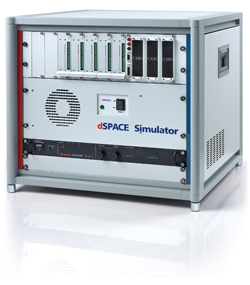
\includegraphics[width=7cm]{contents/images/hil.jpg}
		\caption{Exemple de banc de tests à Continental -- HIL DSpace}
		\label{fig:photoHil}
	\end{figure}


	\subsection{La TA3}
	Actuellement, afin de tester, les équipes de tests disposent d'une plateforme appelé TA3. Cette plateforme leur permet de dialoguer avec des contrôleurs embarqué dans des simulateurs d'environnement\footnote{Hardware In the Loop (HIL) par exemple} et le debugger, et ainsi d'effectuer des scripts de tests en Python.
	\begin{figure}[H]		
		\centering
		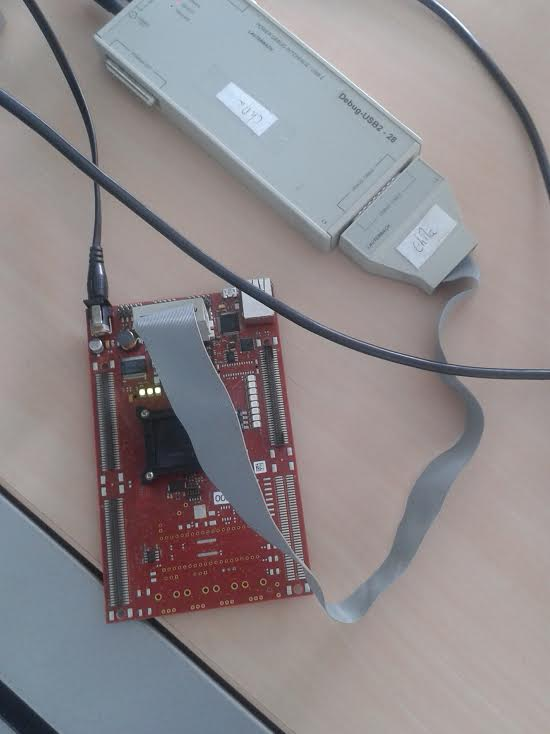
\includegraphics[width=7cm]{contents/images/t32.jpg}
		\caption{Exemple de Debugger à continental -- Trace32}
		\label{fig:photoHil}
	\end{figure}

	Cependant, cette plateforme pose un certain nombre de problème qui rends sont utilisation difficile.
	\begin{description}
		\item[Problème de temps réel] Un certain nombre de calculs à des fins de tests sont effectués par le calculateur, ainsi les tests peuvent être faussés car le calculateur n'est pas en conditions rééls mais utilise une partie de sa charge afin de tester.
		\item[Mauvaise gestion des exceptions] Un autre problème récurrent, est la gestion des exceptions et erreurs de scripts. Cette plateforme utilise python et est donc interprété. Certaines erreurs de syntaxe ne sont détectés qu'à l'exécution : éventuellement plusieurs minutes après avoir écrit le test. D'autre part, certaines erreurs sont inexplicables
		\item[Bugs] Enfin, celle-ci est buggé, il peut arriver qu'elle renvoi des faux positifs, faisant perdre un temps considérable
	\end{description}
~\\
	Il est donc extrêmement difficile de tester dans ces conditions, et celles-ci ayant été mal conçue, il est compliqué de la modifier ou de la faire évoluer. En effet, le résultat serait une plateforme toujours instable, ou alors passer énormément de temps pour un résultat qui ne serait pas parfait : une nouvelle solution partant de zéro afin d'effectuer des tests fiables, simplement et efficacement semble nécessaire.

	\section{La solution : \textit{\textit{GreenT}}}
	Afin de résoudre les problèmes vus section \ref{pbTests}, une solution à été pensé avant mon arrivée en étudiant les besoins de l'équipe en charge des tests du plugin : le développement d'une plateforme de tests, appelé \textit{GreenT}.

	\subsection{Génération de tests automatiques}
	\subsubsection{Les tests d'intégration du plugin Ford}
	A court terme, cette solution devrait permettre de tester le plugin pour les projets Ford facilement et de façon efficace. Pour cela, les testeurs Continental vont ajouter des colonnes dans le document Walkthrough, afin de spécifier la manière de tester les variables. Et la plateforme, sera capable d'analyser le Walkthrough, et de générer les tests automatiques. Le testeur n'aura plus qu'à lancer l'exécutable le soir, il reviendra le lendemain, tous les tests auront été exécutés avec un rapport détaillé pour chaque test.\\

	Ces tests s'effectueront sur des variables enregistrés lors de stimulation du contrôleur, afin de vérifier que celui-ci réagit de façon approprié.

	Cette plateforme permettra donc de tester facilement la dizaine de projets Ford, et une fois le test d'une variable spécifié, il n'est plus nécessaire de le réécrire, à chaque nouvelle release il suffira de relancer les tests : l'équipe n'aura à faire le travail qu'une fois, ensuite la réutilisation sera possible, les projets seront testés plus rapidement, plus efficacement, et plus souvent.

	\subsubsection{Les autres projets}
	A moyen terme, cette plateforme pourrait être utilisé pour les projets d'autres clients tel que Renault, afin d'effectuer là aussi des tests d'intégration, il est donc nécessaire de concevoir une plateforme qui puisse évoluer facilement, et avoir un fichier de spécifications en entrée qui soit légèrement différent d'un client à l'autre.

	En effet, les autres clients peuvent aussi fournir une partie du logiciel, avec un document de spécifications des variables, celui-ci ne serait pas totalement identique, mais l'approche des tests s'en approchera.

	IL est également envisageable que la plateforme soit utilisée pour des tests d'intégration en interne, indépendamment des spécifications fournis par le client.

	\subsection{L'utilisation de \textit{GreenT} comme une bibliothèque}
		Une autre approche de notre plateforme, serait de s'en servir afin de facilement écrire ses propres tests en Java, de façon plus efficace et plus robuste qu'avec la TA3 : notre plateforme doit donc également fonctionner comme une bibliothèque sans utilisation de générateur ou de parser, à la charge du testeur d'effectuer un test rapide. 

		Celui-ci apprendra à se servir de la plateforme, écrira en règle général des tests assez courts et moins complexes que ceux que nous générerons, ceux-ci doivent être faciles à écrire.

	\subsection{L'exécution des tests}
	A long terme, l'objectif serait de pouvoir effectuer de l'intégration continue. 

	Il faut savoir que le lancement de ces tests pourrait durer une quinzaine d'heures, en espérant que l'exécution des tests tienne sur une nuit. Cependant, il va arriver que les tests débordent et que lorsque le testeur revient, les tests ne soient pas terminés : le banc va être occupé alors que d'autres personnes en ont besoin, et le testeur n'a toujours pas les verdicts.

	 Nous souhaitons concevoir un système permettant l'exécution des tests sur des bancs en parallèle : on pourrait ainsi diviser le temps d'exécution par 2 ou 3, ainsi les tests tiendront sur une nuit et l'objectif principal serait tenu.

	 Mais le plus intéressant, serait d'utiliser le décalage horaire à notre avantage : lancer l'exécution des tests sur des bancs non utilisés dans d'autres pays, ainsi à toute heure de la journée il serait possible de lancer les tests. En effet, Continental étant présent dans la plupart des continents, il fait toujours nuit à un site sur la planète. Ainsi, après chaque étape d'intégration, on pourrait relancer les tests afin de vérifier qu'aucun bug n'a été introduit : le problème de la disponibilité des bancs serait alors résolu, et nous atteindrons une excellente sécurité.

